\documentclass{tufte-handout}

%\geometry{showframe}% for debugging purposes -- displays the margins

\usepackage{amsmath}

% Set up the images/graphics package
\usepackage{graphicx}
\setkeys{Gin}{width=\linewidth,totalheight=\textheight,keepaspectratio}
\graphicspath{{graphics/}}

\title{Virtual Labs for Learning, Curating, and Research in Hindustani Classical Music}
\author{Tejaswinee Kelkar,
 Venkatesh Choppella}
\date{28 May 2015}
\usepackage{booktabs}
\usepackage{color}
\usepackage{units}

\usepackage{fancyvrb}
\fvset{fontsize=\normalsize}

\usepackage{multicol}
\usepackage{lipsum}

\newcommand{\doccmd}[1]{\texttt{\textbackslash#1}}
\newcommand{\docopt}[1]{\ensuremath{\langle}\textrm{\textit{#1}}\ensuremath{\rangle}}% optional command argument
\newcommand{\docarg}[1]{\textrm{\textit{#1}}}% (required) command argument
\newenvironment{docspec}{\begin{quote}\noindent}{\end{quote}}% command specification environment
\newcommand{\docenv}[1]{\textsf{#1}}% environment name
\newcommand{\docpkg}[1]{\texttt{#1}}% package name
\newcommand{\doccls}[1]{\texttt{#1}}% document class name
\newcommand{\docclsopt}[1]{\texttt{#1}}% document class option name

\begin{document}

\maketitle% this prints the handout title, author, and date

\begin{abstract}
\noindent This document is a proposal for a Virtual Lab for Music. 
This is a web-based application to provide anybody who is interested in Hindustani music a broad and comprehensive resource containing live experiments to test and hone their abilities; repositories to refer to and obtain material from; and all this in a way that enhances a multi-modal web experience across many domains within music.
In this document, we describe the motivation behind setting up such a lab, the model of integrating experiments, repositories and semantic connections as a complete way of setting up a learning experience that will benefit not just learners of Hindustani Classical Music (hereafter referred to as HCM), but also will function as a resource for other applications such as computation and cognition of music.
\end{abstract}


\section{Introduction}\label{sec:introduction}

Research in music and other arts is important from the point of view of science, arts as well as the humanities. Different areas in human cognition are benefited from musical study, as scientists have found from conducting various types of research. Music is closely aligned with mathematics, literature and poetry from the ancient times. It is also an important method for communities coming together. The study and discipline of music has always been interdisciplinary, but in the modern times we find music to have become more isolated from interdisciplinary research in India. Musical education isn't a necessity in the scope of primary education in India; but over the years, the nature of music as well as musical education is changing. Modern technology is slowly reflecting this change by catering to the needs of musicians.

Technology can participate even more to cater to the changing needs of pedagogical construction, and not just information delivery. Our primary motivation behind building this platform is to bring Indian music education to the web. Music education in India has undergone a revolution in the last century. From being a form that required years and years of apprenticeship with gurus, it has become a form in which remote media of content delivery have become more and more popular. Education delivery online is becoming more and more popular on the web with the arrival of digital libraries, MOOCs, and other forms. Musical education is following some of these patterns, with many repositories for material and an increasing number of people taking lessons over video conferencing and so on. Indian music is only catching up with these trends. The repositories for Indian music are non unified and the teaching methods are not innovative. Technology has mostly contributed only to the medium of delivery, and not the pedagogical methods. 


We propose an on-line learning resource and repository for Hindustani Music. We propose some new methods to bring up a single resource including experimentation and learning, repositories, and semantic linking. We also explain some implications of this on the field of musical research as a whole. Scientifically informed methods of teaching and learning music could greatly improve and inform musical experiences and diversify musical material. 

\begin{marginfigure}%
  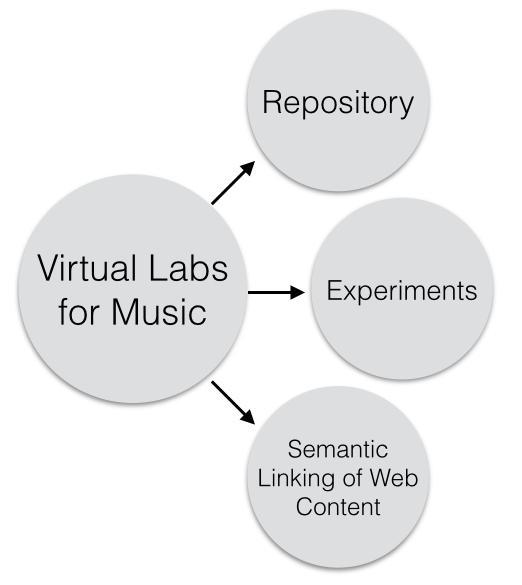
\includegraphics[width=\linewidth]{fig1.png}
  \caption{Sections in the Virtual Labs}
  \label{fig:marginfig}
\end{marginfigure}


\subsection{Review of Related Work}
Music education technology is an upcoming field, with new techniques being tried to address specific challenges \cite{wei2011investigating}, \cite{ccards}, %\cite{phon2005interactivities}, \cite{tambouratzis2008vemus}, \cite{kuuskankare2010pwgl} 

exploring interactivity and openness. Some platforms deal specifically with traditional music education delivery \cite{lou2009study}, while some websites are built for openly introducing music theory in various genres \cite{openmusictheory}. These include sheet music repositories for Western Classical Music \cite{IMSLP-petrucci}, Jazz and Folk collections \cite{smithsonian} and others.  

There are resources that help practice ear training skills \cite{eartr}, or provide databases for compositions from different time periods, lyrics of arias, and other musical material.

Resources for Hindustani Classical music (HCM) are, on the other hand, scattered and disorganised.  Repositories do not cite sources and authors \cite{sra,ncpa}. Popular blogs \cite{parrikar,deepakraja} do not serve as repositories, but merely as opinion delivery, despite careful content aggregation.  Youtube videos form a sizeable chunk of the material available for listeners, although this material is often poorly annotated and described even for basic parameters like composer, raga, taal and other features.  Some websites have repositories skewed towards vocal music alone \cite{swarganga} and keep their services available only for sale.


\subsection{Changing Modes of Pedagogy in HCM}\label{sec:pedagogy}
Hindustani Music traditionally evolved as an art form requiring years and years of guided practise. In ancient times, students of classical music would spend several years with their teachers studying under their scrutinized guidance and slowly absorbing the intricate nuances of the musical performance from the guru. \cite{neuman} Artists were often patronized by princely states and kings and taught students in this system called the \textit{gurukul} system. This started to change towards the end of the 19th century when music reform and education were taken up as a cause by several conferences of music and scholarly musicians of the time.\cite{newmansions} At the time of reform of Indian universities, musical education paradigms changed drastically and musical education was restructured to fit the bounds of a degree education. This meant that the years that could be spent on slowly cultivating musicality and other skills needed to be condensed in a much shorter span. The pedagogical methods changed and the restructuring of courses around study material was a huge challenge of the times. As the twentieth century progressed, both these modes of learning - the traditional way and also the way of classes and tuitions - grew side by side.

\subsection{Twenty First Century}After several changes in musical education, we now have come to the time when musical content is delivered in these two different ways, depending upon where the student goes to learn. One, where gurukula system is heeded and followed, and students get a chance to spend a large amount of time with their teachers and in learning. And another, where music is studied in shorter non-individual lessons. 

A large number of students study within the construct of a classroom, learning with many peers. Lessons are usually structured to be once in a week, and the students are expected to prepare a lot of material by themselves with un-aided, unaccompanied practise. This means that several critical skills, that earlier were absorbed by students offline, by listening to music, are now expected to be naturally developed by them through their own practice. This calls for students being able to arrange for their own practise without the presence of other musicians. 

This challenge can be addressed in two ways. Modern electronic instruments have been invented as replacements for accompaniment in the last twenty years, aiding musical practise greatly. Electronic Tanpura, Tabla, Lehra and Shruti box are now commonly seen not just in practise settings but also on the performing stage. 

Unaided practise also requires engaging methods and tools to aid different ways to develop musicianship. However, the methods of learning musicological concepts haven't been truly exploited through electronic and computer methods for Indian Music. There is no comparable development in music learning applications for students of Hindustani Music to the presence of electronic music instruments. 

Music education must condition itself to the available resources of the students from the overwhelming pressure to cope with other disciplines in scholastic education. We see a rise in music study offered over phone calls, internet voice and video calling \cite{sma}. When students are taught in person, the classes are not more than an hour long. These classes are often taught in groups, where teachers' attention to musicianship of individual students is difficult. Rich multimedia technology still needs to enter the purview of education in HCM, as the sources of education and musical creation through technology, using the theoretical advancements of HCM are almost unexplored. Some websites are made to look more like databases \cite{swarganga}, and this makes the musical study non-interactive.

One of the challenges presented in relying on self learning methodology is the relative lack of reliance on notation systems. Self learning is also aided by the creation of repositories for listeners that are organized based on not consumer oriented, but musician oriented classification ontologies. Virtual Lab for HCM aims to bring change to pedagogy in the ways required rather than letting technology just be a medium. 

\subsection{Notation and Repositories} V N Bhatkhande developed a comprehensive scheme for notation of classical music in the early 1900s. \cite{bhatkhande} His contemporary, V D Paluskar developed a parallel style of notation which is slightly similar to Bhatkhande's. Since then, there have been several notation systems that extend these and bring out more nuances. Bhatkhande's system remains to be the most popular one and is widely used. This has changed musical study greatly. It is now common practise now for students to write the new compositions they have been taught. Composing new structures on paper first is also exceedingly common. However, there haven't been comprehensive and accessible repositories of such music that are available to everyone. Resource books that contain western notations of HCM have also been produced for reference and learning. \cite{kauffman} \cite{ragaguide} Most of this music is written so long ago that it is sung simultaneously in different ways across several \textit{gharanas} and several different composers at the same time, and all of these renditions and years of practise have lent their own modifications to those compositions.\cite{jairazbhoy} New students of music often learn to compose their own music by writing down, in this form of notation, their own drafts of improvisation and so forth. 

Several scholars dismiss notation and writing down, saying that Hindustani Music is meant to be assimilated and never written down. Despite this insistence, it is important to acknowledge the social changes that have led to a changing paradigm for musicians and music learners, who study music through passing on written material.

\begin{marginfigure}%
  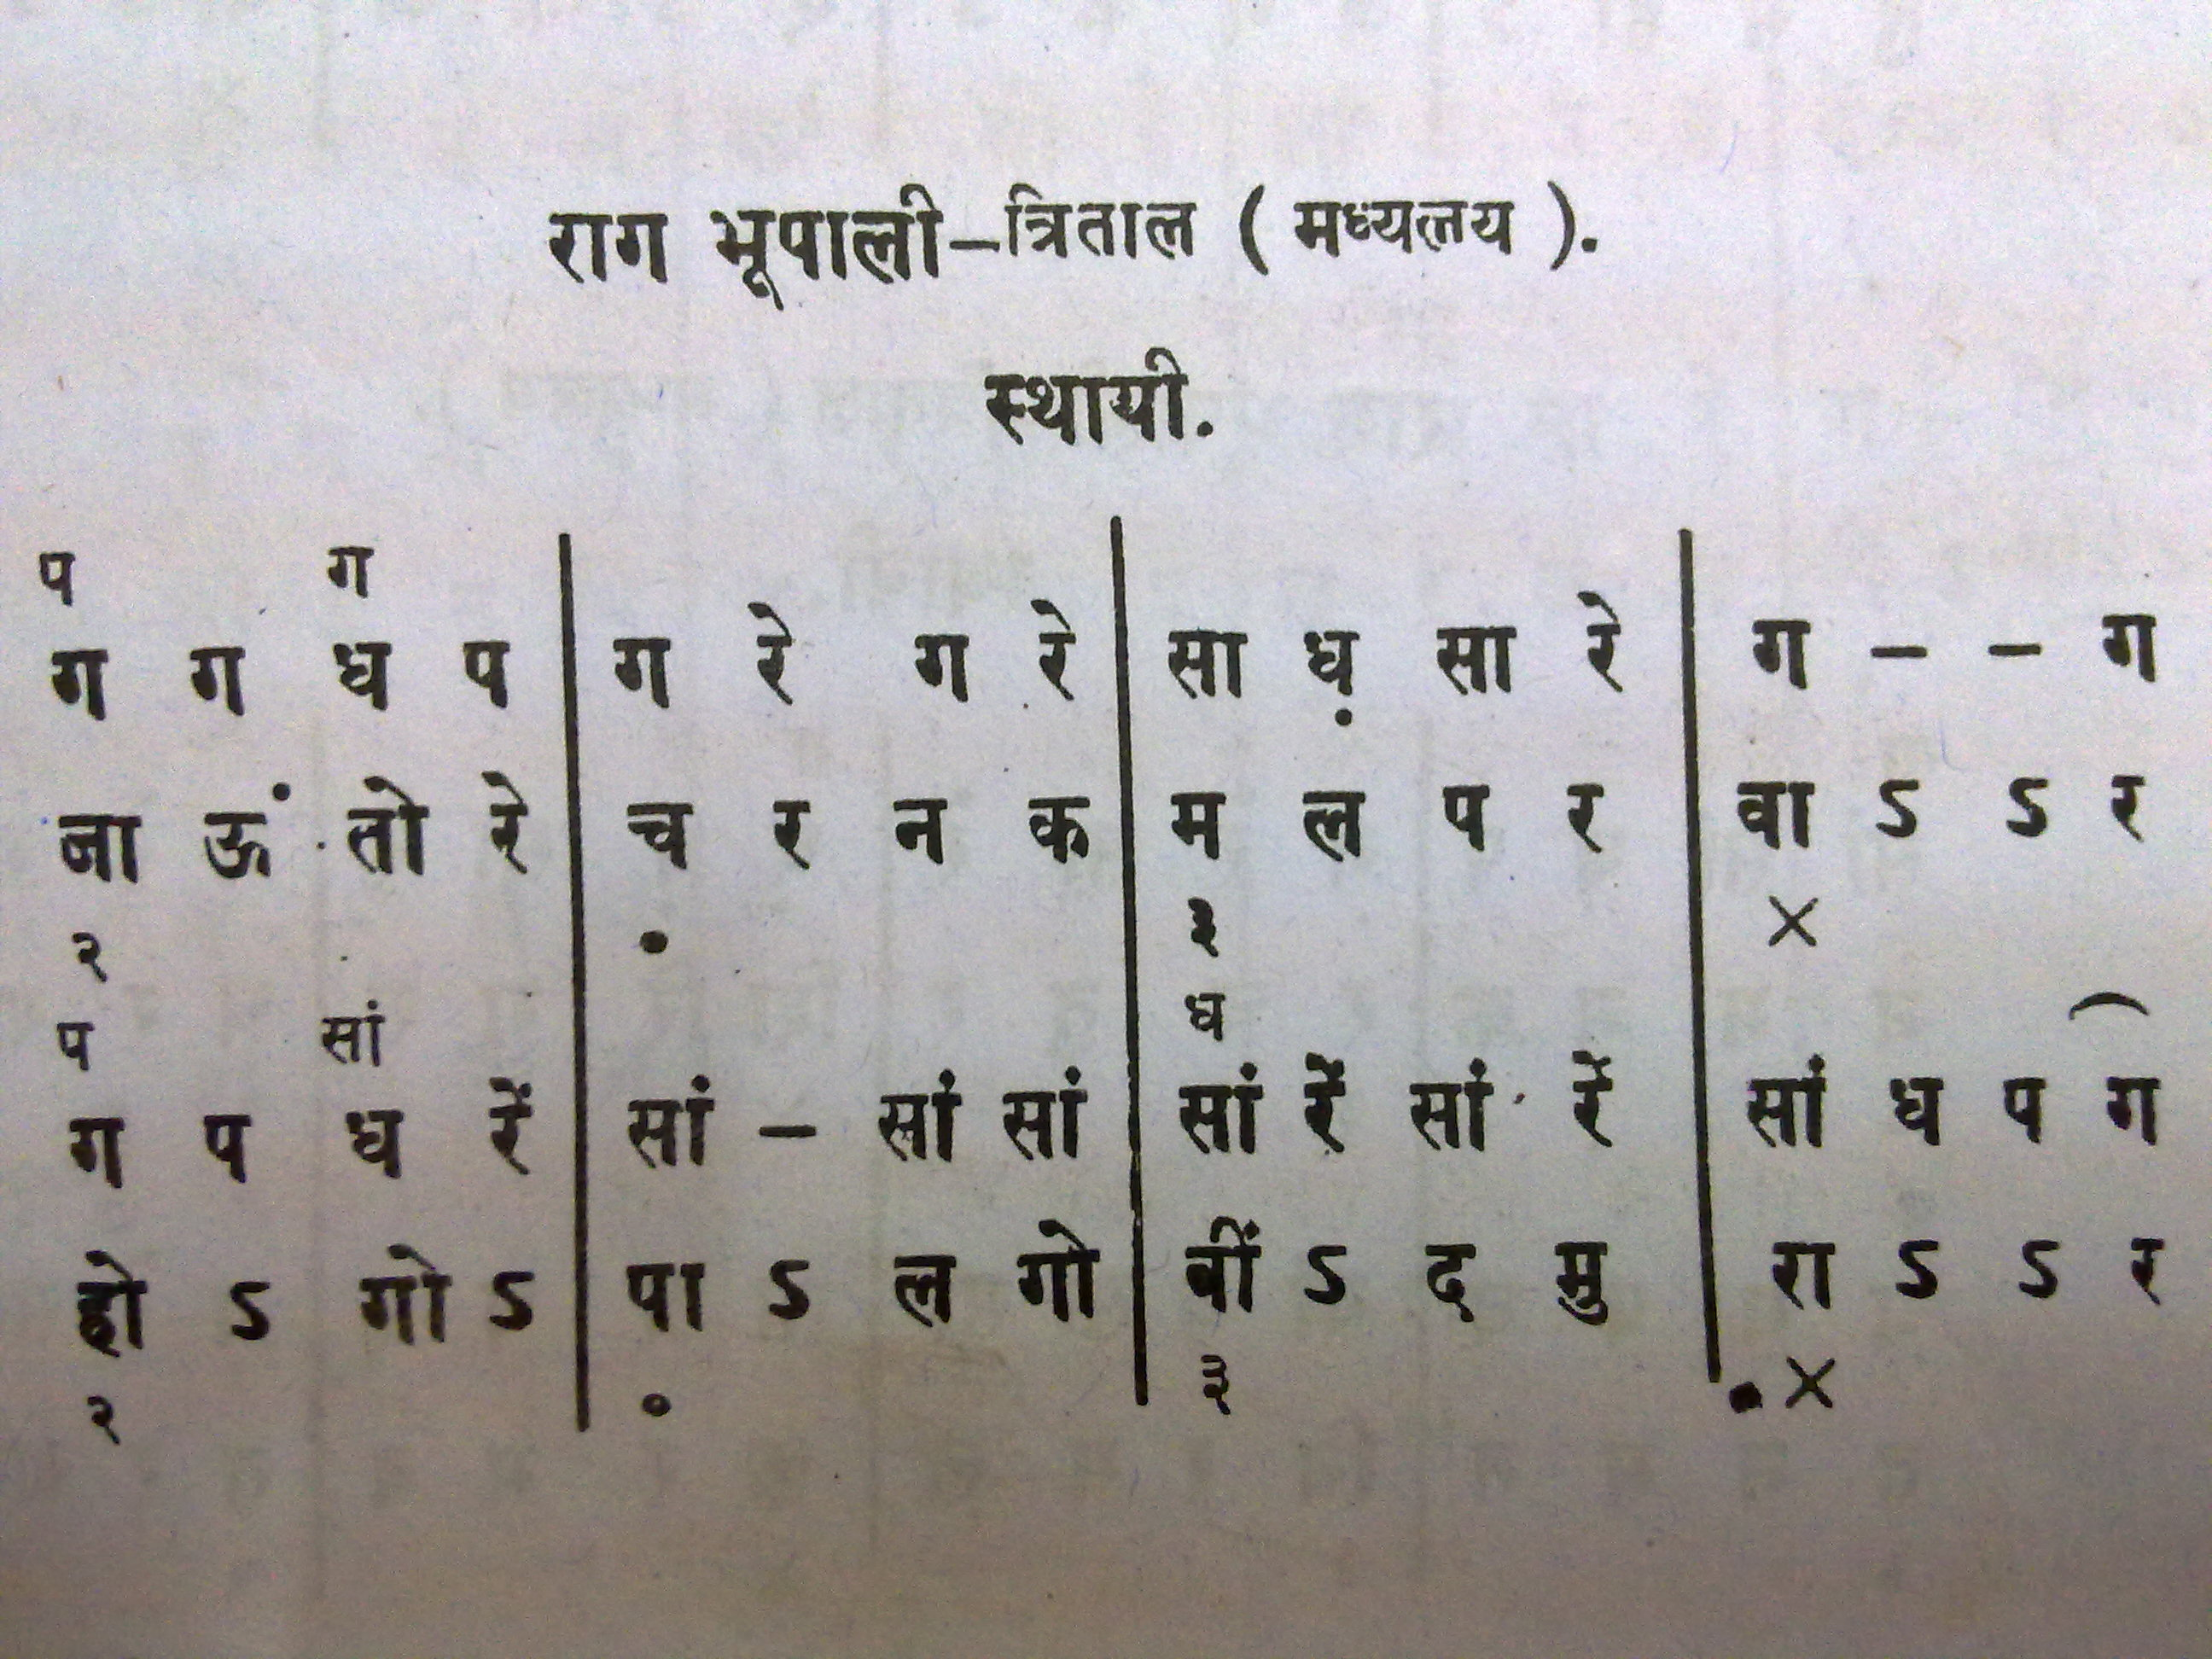
\includegraphics[width=\linewidth]{bhatk1.jpg}
  \caption{Sections in the Virtual Labs}
  \label{fig:marginfig}
\end{marginfigure}


\subsection{Cultivation of Musicianship skills} Critical musicianship abilities are a prerequisite for becoming a learned singer in HCM, just as other systems of classical music. These include the ability to identify notes and note names from hearing music. A musician is expected to be able to identify and notate rhythm, to be able to work with laya, to be able to be a good presenter and so forth. All proficient performers are expected to be comfortable with these skills. For vocalists who don't play an instrument, for instrumentalists who don't sing or aren't required to notate, this task is challenging. Without guidance, through pure listening, these skills take years to come to grips with \textit{Swar-Jnyan} (Knowledge of pitch). Another area that is typically required and often very hard to develop is the proper knowledge of intonation. Hindustani Music uses microtonal scales, and something as simple as tuning a \textit{Tanpura} requires immense expertise and very finely developed ears. It typically takes students years to master this if they are taught. If they are never taught these skills, which happens many a times in tuition-class like model of teaching Hindustani music, these skills remain undeveloped. This challenge is faced by several new students who study music using new methods such as reading from texts, learning with teachers over the internet and so forth. These abilities need to be developed and taught in new way. 

\subsection{Propositions for Novel Methods to introduce musical material}
We take a tripartite approach towards archiving, learning and distribution of classical music. This includes both musicians and non-musicians being able to experiment with music in all capacities. The experiments will enable musicians to be able to engage with experiments to hone their musical skills as well as understand finer and finer nuances of musical listening. 
\paragraph{Power of Practise based methods} We propose a practice based approach towards learning these critical skills of musicality. Battery of tests and a system adapting to the ability level of the student is what is needed in such a case, for teaching these specific skills to students. 

\section{Computational and Cognitive Aspects of HCM}
Computational research in musical creation and cognition have become established fields for study of music in pedagogy, therapy and for its cognitive effects. This approach towards the study of music is becoming popular even for Hindustani music, and has tremendous applications for use in pedagogical, and educational contexts. The forms and function of music beyond its aesthetic value, its contribution to other cognitive systems such as visuo-spatial abilities, language learning potential and so on. Systematic studies regarding Hindustani music could become easier after systematizing the methodology for musical categories, and ease in recording and analysing the performance of a general population in different music-related abilities.  

Virtual lab for HCM also aims at being a platform from which research work with regards to these various aspects of cognition and computation could be carried out easily. Facilitating this, will be the base ontologies that classify and categorize different sound stimuli through annotation, and other methods. This will help datasets to be readily available for people to prune and analyze or transform. 

New experiments that require large amounts of data to be collected can also be easily performed on this platform. Some examples are: understanding the generation of mood of
\emph{rasa} or \emph{raga}, pedagogical
methods to enhance learning and practice, generative
structures of raga and so on and so forth. It would also be
an important task in this project to generate a formal
ontology of Hindustani music which would make it easy to
understand not only the structures of music, but also
meta-tag and retrieve more data from the new musical uploads
that are generated.

These new fields can aid hugely, our understanding of music as a cognitively essential art. 

\subsection{Our Contributions}
We can classify music education resources in the following general categories: 1. experiments and drills for sharpening skills, 2. repositories for crowdsourcing or hosting information, and 3. linking music and creating opinion based resources. 

Virtual Lab for HCM (\texttt{http://music.virtual-labs.ac.in}) is a platform reflects a mix of all three streams mentioned above. It is an open, interactive and networked self-practicing environment for education in HCM, that enables users to experiment with musical concepts on an on-line platform. It supports musical education by tailoring to a new model of pedagogical delivery that has not been used in the context of HCM before. This includes the creation of several drills and exercises for musicianship skills, visualization alternative descriptions of several aspects of music theory. This platform helps create a community driven architecture that allows users to be contributors of content. Not only can users learn, browse and annotate content from their own musical knowledge, but also share this with other users. Unlike other platforms of this kind, Virtual Lab for HCM can then use the sounds annotated by others in creating and structuring its own experiment stimuli and examples. This  opens up a large volume of musical content to be available as study material - both in the form of audio annotations and descriptions. This feature makes Virtual Lab for HCM unique.


\section{Virtual Lab for HCM as an Open Architecture}

\subsection{Features of the Open System}
\begin{marginfigure}
\centering
    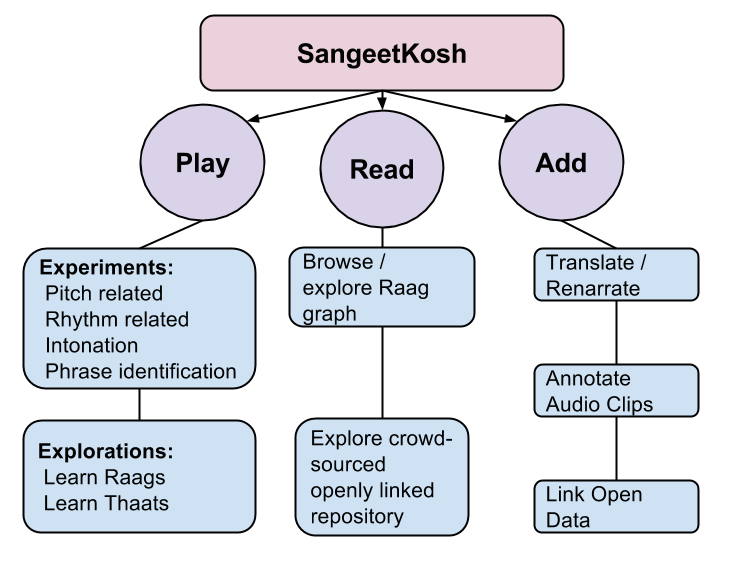
\includegraphics[width=0.8\textwidth]{threeprong.png}
\caption{Three pronged structure of the lab}
\label{fig:opensystem}
\end{marginfigure}

Virtual Lab for HCM has a three faceted structure for its architecture. The first facet deals with the musicianship skill building - including tests on ear training of pitch, rhythm, notation. The second facet deals with theoretical explorations such as learning concepts of \textit{raga}, \textit{taal}, \textit{thaat} - which are necessary for education in music as well as the exploration of theory. The third facet deals with the linking and simultaneous presentation of these various concepts through user contributions, annotations and translations. In figure \ref{fig:opensystem}, these three facets are explained as 'play', 'read', and 'add'.

Most websites offering self learning of ear training present methods to turn musicianship skills into games and drill exercises using fixed, generated or predetermined stimuli or set of stimuli. In section II. B, we will also present an architecture to expand this selection to picking sound samples from other sources on the web. This feature makes this platform unique as against others.


\subsection{Play: Experimenting with musical Concepts}

The first facet of Virtual Lab for HCM is in allowing people to experiment with musical concepts, and to practise and play with music theory. Typically musicianship is developed as a by product of years of practise. In the current model, some students find practice challenging because of not being able to play an instrument, and therefore have reference notes. Initially, it is also harder to formulate a good understanding of taal concepts in practise. There are other musicianship challenges faced by students from time to time, including - knowing what written music sounds like by playing it, learning the right tuning or intonation to fine tune their instruments, learning how to count rhythm and compose their own phrases, and many others. We present a series of experiments that will let users practise these focussed tasks in the form of a game. This ensures that users can practise and get feedback on a machine, and can therefore continue practising for as long as they like.

\begin{marginfigure}
\centering
    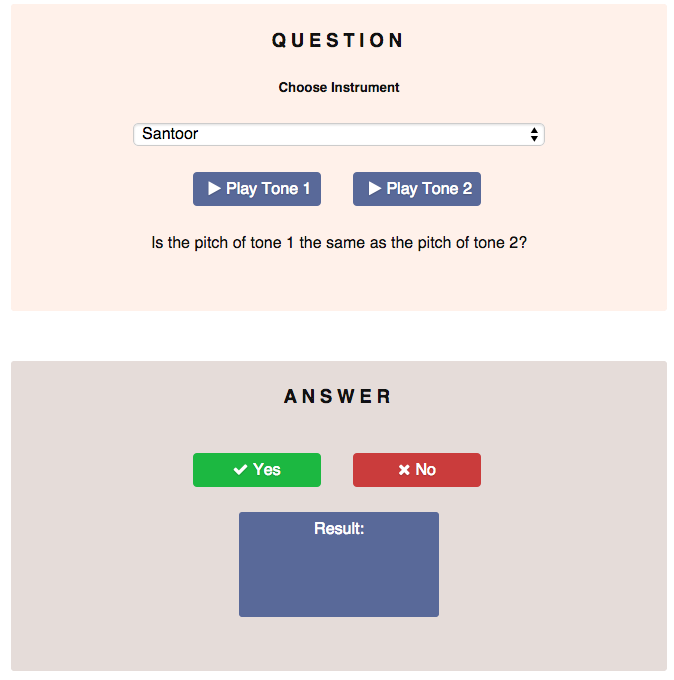
\includegraphics[width=0.8\textwidth]{expt1.png}
\caption{Example of an Experiment}
\label{fig:experiment}
\end{marginfigure}

An example of the experiment interface can be found in Fig  \ref{fig:experiment}. The system is designed to be able to pose questions in several Indian instruments, making it adapt to the specific needs of the musical system. 

\subsection{Read: Content Aggregation}
The second feature of this platform is to provide content and repositories for students of music. HCM involves extended musicological and theoretical material that students must learn and know. For this, we need a place where compositions, theoretical instructions and nuances, and source material can be read. We start with a base ontology containing the theoretical structures of HCM. This ontology is derived from authoritative books of music theory \cite{bhatkhande, kramik}. Making this ontology open for navigation and exploration condenses several pages of dry theory into a succinct, interactive interface.

As seen in Figure \ref{fig:onto}, we create a graph for linking and establishing the minute features of the musical categories like ragas, their classification and constituents. This serves as an ontology from which the repositories can be accessed. We populate this resource by opening it for linking with other media on the web or openly adding or uploading other resource material, as explained in section II B.
  
  
\begin{marginfigure}
\centering
    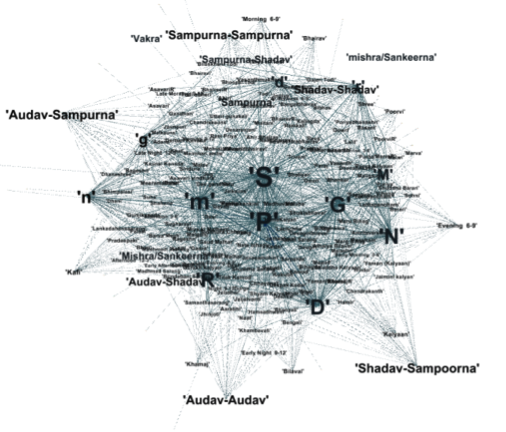
\includegraphics[width=0.8\textwidth]{graph.png}
\caption{Raga Graph - Base Ontology}
\label{fig:onto}
\end{marginfigure}

\subsection{Add: Annotation and re-narration of web content}

Music experiment platforms typically use their own midi modules or sound clips in order to generate the testing questions \cite{tambouratzis2008vemus}. This limits the musical material produced by the system to be restricted to just a few musical instruments. Some teaching softwares use scoring support \cite{kuuskankare2010pwgl}, which is not used in the study of HCM. Midi modules support more western instruments rather than indigenous Indian instruments. Open annotation and re-narration solves this problem by allowing a content creator to contextualize a newly uploaded sound file, by providing attributes for it. When the file needs to be sourced to use as a stimulus, it can directly be used by referring to its attributes rather than requiring the data to be stored on to a server while using them in experiments and quizzes. 

Adding musical material and annotating it is also a task that can be performed by  users who may or may not be content creators. This opens the platform to the web in a unique way, described as follows.

\section{Open Linked Data to Connect Music Resources}
\begin{marginfigure}
\centering
    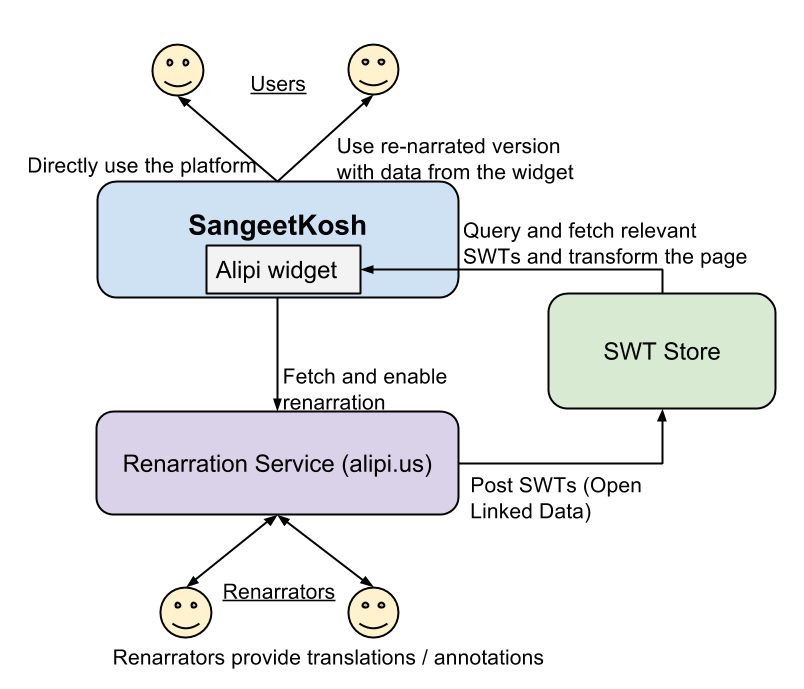
\includegraphics[width=0.8\textwidth]{alipi.png}
\caption{Diagrammatic representation of the architecture}
\label{fig:verticalcell}
\end{marginfigure}


Virtual Lab for HCM is designed as a modern HTML5 application, leveraging
 HTML5 standard APIs so that rich multimedia and interactive content
can be delivered through an open platform. The architecture of Virtual Lab for HCM can be seen in Fig \ref{fig:verticalcell}. We construct an architecture to use decentralized locations that store messages, through a set of tools that we call the Alipi Tool Suite (ATS). The ATS contains several small tools within it to augment Virtual Lab for HCM and facilitate linking openly available resources on the web. More description of the ATS can be found in \cite{prasad2014overcoming} \cite{dinesh2012alipi}.

ATS uses Semantic Web Tweets or SWTs, which is a way to structure and store decentralized, social semantic web tweets. A SWT  is a small message generated in the process of linking and annotation. The anatomy of a SWT is as follows:

@user \#context /resource {attributes}

It is a structured message that is stored openly on the web. Information is stored in the following way:
\begin{enumerate}
\item The author of the SWT (or linking open data),
\item The context of the SWT,
\item The URI of the resource,
\item The attributes provided by the user. Context determines what attributes can be present.
\end{enumerate}

The ATS tools publish SWTs to a decoupled SWT store, which not only stores but also provides a query interface. The SWT store is queried for the relevant information to be displayed once the user logs in. The application also uses a re-narration service called Alipi hosted at \texttt{http://alipi.us} \cite{alipi}. ATS tools provide the following services that assist the operations of Virtual Lab for HCM:
\begin{enumerate}
\item Annotation: This enables a user to add new information to an existing web page.
\item Translation: This is a direct translation into a different language
\item Re-narration: This is a narration of existing content to a specific context, such as re-narrating a jargon heavy document into a simple language and so on
\end{enumerate}

We describe how each of these tools are used as follows: 

\subsection{Audio Annotation tool} 
\begin{marginfigure}
\centering
    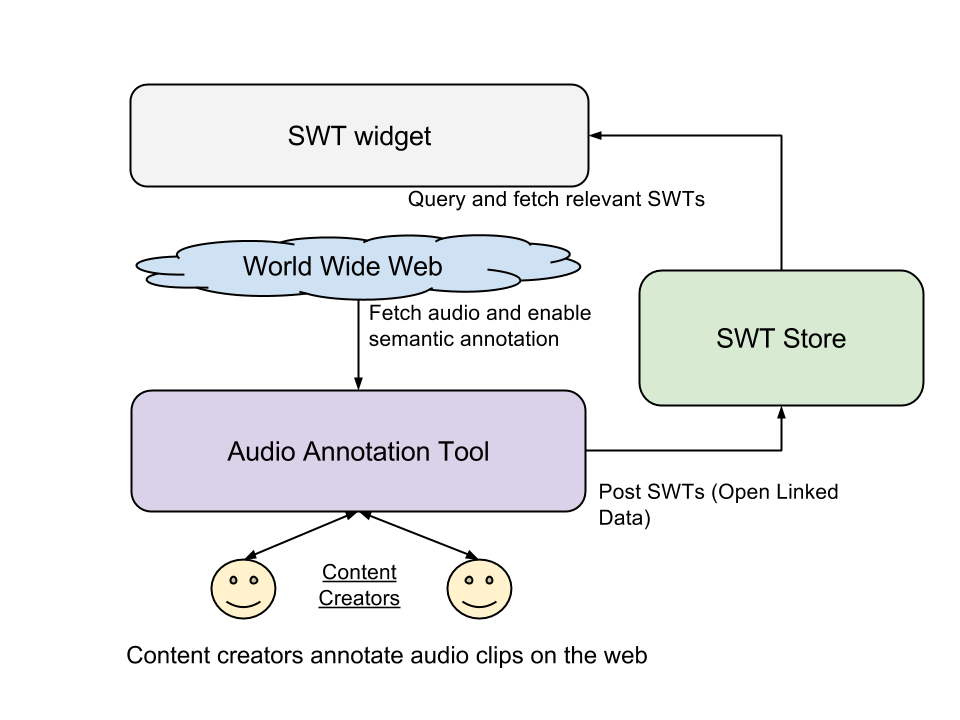
\includegraphics[width=0.8\textwidth]{audioanno.png}
\caption{Architecture of the audio annotation tool}
\label{fig:annotation}
\end{marginfigure}
This is a web-based application which provides an easy
interface to annotate an audio clip to add musical information to it.
For example, the user can annotate the stresses in a musical bar, or the
properties of a musical phrase and so on. This information can be used to query and retrieve phrases which all have the same property. These audio clips can exist anywhere on the web, as long as they are freely and openly available, they can be annotated using this tool. After annotation, the tool sends a SWT containing the annotated information, and the URI of the original resource, and posts it to a SWT store. For example, tabla sound clips from Freesound \cite{akkermans2011freesound} can be used by a content creator to annotate to stresses or rhythm information. As the embedded tool that understands the semantics of the annotation, it can then be used by the Virtual Lab for HCM in a particular drill or quiz. The architecture of this application can be seen in Fig \ref{fig:annotation}.

\subsection{Translations through Alipi} Users can contribute alternate translations of the content in other languages by using the ATS.  To use the service, re-narrators navigate to the Alipi website \cite{alipi}, and request for Virtual Lab for HCM. Then the service fetches the website and present them with an interface through which they can browse it, point-and-click on the content
to bring up an editor, and contribute alternate narratives
or translations.

An Alipi widget is integrated with the Virtual Lab for HCM. This widget fetches 
re-narrations of a particular language, based on user preferences and transform
the page accordingly. The content creators can recognise a set of authors whose
re-narrations can be used to provide alternate translations for the Virtual Lab for HCM. This makes translations fast, and easily accessible, and also enables anybody to contribute and share translations as they like.

\subsection{User Annotations / Re-narrations} Another tool in the ATS is the 
re-story application (\texttt{http://restory.swtr.us}). This service can be used by
end users to provide alternate narratives and annotations to
the existing content of the Virtual Lab for HCM. It can also be used to
link other resources on the web, like videos, audio clips, and
reading materials, to the existing content of the platform.


\subsection{Crowd-sourcing to re-notate compositions} Available compositions in
Hindustani Music in older textbooks and scripts can be crowd-sourced to
annotate and re-notate. This re-notations can be added to the repository of
information in Virtual Lab for HCM. Upon making these compositions searchable, they add to the databases that can be created using musical documented and notated musical material. 

\section{Cultural and Social Innovations of Virtual Lab for HCM}
The applications of this technology are to specifically address the challenges posed by HCM in the current education system. We explain the challenges of musical education and the ways in which Virtual Lab for HCM addresses them.

\section{Traditional and Modern Pedagogical Methods}
Some of the challenges faced by a web based music education platform in India pertain to the historical methods of education in HCM, while others have to do with the means of technological usage that are most popular. 

HCM traditionally evolved as an art form requiring years and years of guided practise. Until the twentieth century, students of classical music would spend several years as apprentices studying under the guru's scrutinized guidance, slowly absorbing the intricate nuances of the musical performance from the guru. \cite{neuman} Artists were patronized by princely states and kings and taught students in this system called the \textit{gurukul} system. This started to change towards the end of the 19th century when music reform and education were taken up as a cause by reformists and scholarly musicians of the time \cite{newmansions}. At the time of reform of Indian universities, musical education paradigms changed drastically and musical education was restructured to fit the bounds of a college degree. 



\section{Development so far}
As a team of 5-6 developers, over the last six months, we have developed 15 unique experiments designed to help students of music understand pitch, rhythm and instrumentation related concepts. The list of work completed is as follows:
\paragraph{Experiments}
\begin{itemize}
\item Pitch Same or Different
\item Pitch Direction
\item Name the Svar
\item Listen to Sargam
\item Listen to Thaat Categories
\item Name Series of Svar
\item Navigate Ragas visually
\item Identify the Instrument
\item Raga Quiz
\item Taal Quiz
\item Tune two strings
\item Trace a Melody
\item Listen to Taal Bols
\item Identify Baayan and Dahina sounds
\item Listen to Taals
\end{itemize}

\paragraph{Raag and Taal Ontology}
We have created navigable graphical ontologies for Raga and Taal categories. These ontologies contain large datasets spanning most commonly occurring ragas and taals. They have been linked with edges specifying each of their parameters and relationships. this makes these ontologies exhaustive. These ontologies are used to run two parts of the lab:
\begin{enumerate}
\item Ontology driven quizzes
These quizzes are as specified in the experiments section. They help users answer different kinds of questions based on their level of difficulty about raga and taal in HCM. They reflect the examination question patterns in 
\item Ontology driven annotation
The ontologies can drive annotation tools that we are building to link other semantic resources to the lab. These annotations then, can in turn drive more quizzes and experiments, having a virtually unending source from which to obtain stimuli, because we will use sound files on the web that are already uploaded that are free to play.

\end{enumerate}

\paragraph{Other Tools}
\begin{enumerate}

\item \textbf{Annotation Tools: }
We have completed an ontology driven annotation tool to semantically link data that is already present on the web to lab resources. This tool helps provide metadata for those sound files directly, or also annotate parts of it to highlight specific notes or ornaments etc.

\item \textbf{Translation Tools:}
As explained above, translation tools have been implemented to get virtual labs for Music to be available in many different languages that we speak.
\end{enumerate}

\section{Deliverables}
The following will be the deliverables for this project:
\begin{itemize}

\item Experiment Portal\\
This portal will contain a complete list of experiments in two sections:
\begin{itemize}
\item Music Learning Experiments\\
These experiments will be designed for teaching students of music some elements of musicianship and providing them with drills for learning.
\item Music Appreciation Experiments\\
These experiments will teach the users how to appreciate musical nuances and what to look for in HCM.

\end{itemize}
\item Repository\\
This section will contain resource material for popular khyals in HCM, notated. It will also contain the following:
\begin{itemize}
\item Repository of Khyals
\item Raga-Net: A graph visualization of Concepts, Ragas, Gharanas, Artists and so forth in HCM
\item Links between 
\end{itemize}

\item Behavioral and Cognitive Science Experiments for Music\\
\begin{itemize}
\item Analyzing data from demographic - Musical abilities of music learners 
\item Vocalization and native language - How do vocal habits and articulation of the mother tongue language affect and change the singing voice

\end{itemize}

\item Linked Resources\\

\end{itemize}

\section{Timelines}


\paragraph*{}
After obtaining feedback from the users of this portal, the experiments will be updated

\begin{table}[h]
\begin{tabular}{ll}
\toprule
Version 2                    & Contents      \\
\midrule
Experiment Portal & All Rhythm and Instrument\\ & Experiments\\
Repository & Crowdsourcing khyal documents\\
Ontology & Visualization of Raga Ontology\\
& Queriable ontology create\\
\bottomrule    
\end{tabular}
\caption{Version 2}
\end{table}


\begin{table}[h]
\begin{tabular}{ll}
\toprule
Version 3                    & Contents      \\
\midrule
Experiment Portal              & Raga and Khyal relation\\
& related experiments\\
Repository                     & Releasing bandish databases\\
& from collected repositories\\
Ontology & Mapping contemporary compositions\\
 & to ontologies\\
\bottomrule    
\end{tabular}
\caption{Version 3}
\end{table}


\begin{table}[h]
\begin{tabular}{ll}
\toprule
Version 4                    & Contents      \\
\midrule
Experiment Portal              & Gamification of All Experiments\\
Repository                     & Provide a searchable database of bandishes\\
 & Collecting private Bandishes from people\\
Ontology & User Privileges to add \\ 
& content from other sources\\
\bottomrule    
\end{tabular}
\caption{Version 4}
\end{table}

\section{Budget and Resources }
\label{sec-1}
\section{HR}
\label{sec-1-1}


\begin{center}
\begin{tabular}{lrrrl}
\hline
 Item           &   Cost  &       &         &     \\
                &  (L/y)  &  No.  &  Total  &     \\
\hline
 MS Student     &    3.5  &    1  &    3.5  &     \\
\hline
 Engineer       &    4.5  &    1  &    4.5  &     \\
\hline
 Research Asst  &    1.5  &    1  &    1.5  &     \\
 (S/W)          &         &       &         &     \\
\hline
 Total          &         &       &    9.5  &     \\
\hline
\end{tabular}
\end{center}
\section{Equipment}
\label{sec-1-2}



\begin{center}
\begin{tabular}{lrlll}
\hline
 Equipment       &        &     &     &     \\
\hline
 Field Recorder  &   .20  &     &     &     \\
\hline
 Mic             &  0.05  &     &     &     \\
\hline
 Mixer           &  0.15  &     &     &     \\
\hline
 Mac Laptop      &  0.80  &     &     &     \\
\hline
 Total           &   1.2  &     &     &     \\
\hline
\end{tabular}
\end{center}
\section{Consumables}
\label{sec-1-3}



\begin{center}
\begin{tabular}{lrlll}
\hline
 Server hosting  &  0.20  &     &     &     \\
\hline
\end{tabular}
\end{center}
\section{Travel}
\label{sec-1-4}



\begin{center}
\begin{tabular}{lrlll}
\hline
 Visits to            &       &     &     &     \\
 Music Colleges       &    1  &     &     &     \\
 and Museums          &       &     &     &     \\
\hline
 National Conference  &  0.5  &     &     &     \\
\hline
 International        &    3  &     &     &     \\
 Conference           &       &     &     &     \\
\hline
 Total                &  4.5  &     &     &     \\
\hline
\end{tabular}
\end{center}
\section{Total}
\label{sec-1-5}



\begin{center}
\begin{tabular}{lrlll}
\hline
                    &    9.5  &     &     &     \\

                    &    1.2  &     &     &     \\

                    &    0.2  &     &     &     \\

                    &    4.5  &     &     &     \\
\hline
 Total              &   15.4  &     &     &     \\
\hline
 @0.15 contingency  &   2.31  &     &     &     \\
\hline
 Total              &  17.71  &     &     &     \\
\hline
 @0.15 college funds & 2.65 &  &  & \\
\hline
Total 			   & 20.36 & & & \\
\hline
\end{tabular}
\end{center}

\section{Conclusions}
There is thus an immense potential to channel the information in Hindustani music into a computer based resource for education, deepening cognitive understanding of music, as well as developing web architecture that supports the multimodal requirements of musical material.

The lab will support drills in musicianship, fitting into the ever changing pedagogical practises of Hindustani Music. A repository that will also enable computational experiments in extending the bounds of experimentation in Hindustani Classical Music. 

This will be the broadest attempt of its kind to fit the missing pieces together, and will serve as a massive source of information.

\bibliography{sample-handout}
\bibliographystyle{plainnat}

\section{Appendix - Description of Some Concepts Mentioned}

\section{Sample Set of Experiments}
\paragraph{Expt 1 Pitch discrimination}
This experiment will focus on students being able to distinguish
between two pitches that are played consecutively. The students will
only to answer whether the two pitches played are the same or
different.
\paragraph{Expt 2 Pitch Direction}

This subsequent experiment focuses on being able to identify the
direction of difference of the given pitches. After the student is
comfortable telling two tones apart, this experiment will help them
understand whether the subsequent tone is lower or higher than the
first.
\paragraph{Expt 2.5 What are notes?}
This experiment will explain the concept of notes and
octaves. Students will learn to identify octaves and figure out how
notes played in a row sound. Different instruments can be used to
elaborate this. For vocalists, this may include clicking on the names
of svaras / intervals and then listening to them. Students will also
be able to play notes as scales with note names to familiarize with
the concept of naming notes.\\
Before we move to interval identification, this experiment is a free
exploration of musical hearing.

\begin{itemize}
\item 1. Free exploration with instrument and note names

\item 2. Free exploration hearing different scales and note sequences\\
\end{itemize} % ends low level

\paragraph{Expt 3 Pitch identification from same tonic}

Here we start to move to interval hearing and tone training. \\
Before being able to train the ear for identifying pitches, this
simple experiment will help students distinguish between 

\begin{enumerate}
\item Levels
\begin{enumerate}
\item Level 1: Sa, Ma, Pa
\item Level 2: + Ga, Ni
\item Level 3: + Re, Dha
\item Level 4: All Shuddha Notes
\item Level 5: + Re Dha Komal
\item Level 6: + Ga Ni Komal
\item Level 7: + Tivra Ma
\item Level 8: All notes
\end{enumerate}
\item Number of Questions
\end{enumerate}

\paragraph{Expt 4 Pitch identification from separate tonic}
While the tanpura is playing in another key, a different reference
note will be given to judge another pitch interval from.\\
This experiment is to build hearing independence outside the tonic, as may be required in some forms of light classical singing.
\paragraph{Expt 5 Identifying a chain of pitches}
In this experiment, the experimenter will have to name the notes in a row of pitches in a single tonic. This experiment will decelop the knowledge of `svar-sthan' in the users.
\begin{enumerate}
\item Levels
\item Number of Questions per level
\end{enumerate}
     
\paragraph{6 Tabla Simulation}
The goal of this experiment is to simulate a tabla skin on a computer,
and choose and handshape, and simulate the sounds that a tabla makes
if it is struck at different points.\\ 
Understanding tabla bols also requires an understanding of how it is
played on the skin membrane. This experiment will help people who
don't have access to tablas to explore the instrument in detail.

\begin{enumerate}
\item Hearing bol and location of playing
\item Composing new taals
\end{enumerate}
     
\paragraph{Expt 7 Khali and Taali}
This experiment is to explain the polarity between these two events in
Taal. The rhythmic and motional feeling of a downbeat and an upbeat
will be explained. Participants will get to freely explore and listen
to tabla sounds, and figure out the presence of khali and tali in the taals.
\begin{enumerate}
\item Analyzing khali and taali in visual form
\item Building larger metrical structures for khali and tali
\item Splitting These structures into different laya combinations - aad, kuaad, bayaad
\end{enumerate}
\paragraph{8 Singing and melograph plotting}

Dynamic capture of musical voice and generation of melographs dynamically with 

Melographs are a visual representation of the sung music. This
experiment will help people familiarize themselves with a visual
scheme to understand music. This scheme will be taken forwards

\begin{enumerate}
\item Matching own melograph with template melographs
\item Difference measure for melographs
\end{enumerate}


\subsection{Sample Research Questions}

\begin{itemize}
\item Musical Proficiency in General Population\\
There are no real numbers to determine the musical profeciency of a general population. Often, the tests undertaken fail to get contextualized to an ethno-cultural demographic. This portal will enable us to create a space to easily experiment with the data on musical proficiency through the tests built on it.

\item Pedagogical Research on Repetitive Learning\\
What is the best method of teaching somebody to listen to nuances of music? Through this portal, we can try various styles of teaching and see how they perform on an average for a general population.

\item Musical Absorption and Rasa Theory\\
Experiments can be built to check the involvement of musical listeners and musicians in the emotional content as described in the Rasa theory, and to better map it to ragas, raga times and so on.
\end{itemize}
\end{document}
